\chapter{Putting a Price Tag on Life}

This chapter follows Michael Sandel's second lecture in \emph{Justice}, presented here in companion-note form for the LazyLearn track and curated by LazyingArt LLC. We return from the lifeboat case of Dudley and Stephens to Bentham, because the question is no longer only whether one desperate act was justified, but whether there exists a general rule for choosing the right act or the right law. Sandel's answer, at first, is mathematically spare: we add benefits, subtract costs, and choose the larger balance. The entire lecture then asks whether that spare arithmetic is morally adequate.

\section{Returning to Bentham}

Sandel begins by reminding us of the lifeboat case and then stepping back into philosophy. Bentham's thought is introduced not as a detached doctrine but as a candidate explanation of what we were already tempted to do in the lifeboat: count lives, compare pains, and choose the larger good. Bentham's life enters only briefly. The important point is that he devoted himself to jurisprudence and moral philosophy, and that his version of utilitarianism aims to govern both private conduct and public legislation.

\begin{definition}
Bentham's principle of utility says that the highest principle of morality is to maximize the general welfare, or the collective happiness, or the balance of pleasure over pain.
\end{definition}

Sandel states this principle in prose. For compactness we may write it as
\begin{equation}
U = H - S,
\end{equation}
where \(H\) denotes happiness or pleasure and \(S\) denotes suffering or pain. The formula is only shorthand, but it captures the lecture's governing idea exactly.

The next move is essential. Bentham does not restrict this arithmetic to one person's life. He extends it to the community as a whole. A community is, in his phrase, the sum of the individuals who comprise it. In a compact notation we may write
\begin{equation}
U_{\text{community}}=\sum_{i=1}^{N} u_i,
\end{equation}
where \(u_i\) is the contribution of the \(i\)-th person's pleasure and pain to the common total. Once we write the matter this way, the decision rule becomes immediate:
\begin{equation}
a^\star=\arg\max_a U(a).
\end{equation}
The right act, policy, or law is the one that maximizes utility.

This is the first mathematical spine of the lecture. It is not elaborate, but it is exact enough to guide legislation. If we can identify the relevant benefits and costs, and if we can place them on a common scale, then the calculus tells us what to do.

\section{Cost-Benefit Analysis as Utilitarianism in Practice}

Sandel's first major pivot is from principle to administrative practice. He tells us that utilitarian reasoning now often goes under a different name: cost-benefit analysis. The form is the same. We enumerate benefits, enumerate costs, translate them into comparable units, and choose the policy with the largest net gain.

For a policy \(a\), the operational rule is
\begin{equation}
\text{Net}(a)=\text{Benefits}(a)-\text{Costs}(a).
\end{equation}
At this level the arithmetic seems unobjectionable. The question is what happens when we actually populate the ledger.

The Czech smoking case is Sandel's first worked example. Philip Morris commissioned a study of smoking in the Czech Republic. The result, Sandel reports, was that the government gains by having Czech citizens smoke. The ledger runs as follows:
\begin{align}
\text{Net}_{\text{Czech smoking}}
&=\text{tax revenue}
+\text{health-care savings from early death} \nonumber\\
&\quad+\text{pension savings}
+\text{housing savings}
-\text{smoking-related health costs} \nonumber\\
&=\$147\,\text{million}.
\end{align}
And at the level of the individual case, the same logic yields
\begin{equation}
\text{savings per premature death} > \$1200.
\end{equation}

The point of the example is not that the arithmetic is internally inconsistent. On the contrary, the arithmetic is coldly coherent. The point is that something morally grotesque appears the moment we let the ledger run without interruption. Early death becomes a fiscal benefit. The right side of the equation includes tax revenue and reduced pension obligations; the left side includes the costs of disease. The comparison can be done. But should it be done in that way?

At this stage Sandel is careful. A defender of utilitarianism might reply that the Czech study is unfair because it leaves out the value of life itself. If the death of the smoker and the loss to the family were properly entered into the ledger, perhaps the calculation would come out differently. This reply does not yet reject the calculus. It asks only for a fuller and better calculus.

\section{Ford Pinto, Cell Phones, and the Price of Life}

The Ford Pinto case is introduced precisely to test that reply. Suppose, Sandel says, that we do assign a dollar value to life. Does that rescue cost-benefit analysis, or does it deepen the problem?

Ford knew that the Pinto's rear fuel tank was vulnerable in collisions. The company estimated the cost of a safety improvement at \(\$11\) per vehicle, applied across \(12.5\) million cars and trucks:
\begin{equation}
C_{\text{Pinto safety}}=(\$11)\cdot(12.5\times 10^6)\approx \$137\,\text{million}.
\end{equation}
The benefit side of the memo, as Sandel narrates it, counted expected deaths, injuries, and destroyed vehicles. Because the transcript compresses the injury coefficient, it is best to keep that term symbolic:
\begin{equation}
B_{\text{Pinto safety}}
=
180(\$200{,}000)+180I+2000(\$700)\approx \$49.5\,\text{million},
\end{equation}
where \(I\) is the injury valuation implicit in the memo.

The decision rule is then immediate:
\begin{align}
\Delta_{\text{Pinto}}
&=B_{\text{Pinto safety}}-C_{\text{Pinto safety}} \nonumber\\
&\approx \$49.5\,\text{million}-\$137\,\text{million} \nonumber\\
&\approx -\$87.5\,\text{million}.
\end{align}
On this calculation the safety device is not installed.

This is a genuine worked example of utilitarian policy reasoning. It is not merely an intuition pump. The magnitude of the quantities governs the decision. And yet, as Sandel emphasizes, the jurors were appalled when the memo emerged in court. The memo had included a price for life. The scandal, then, cannot be explained simply by saying that life had been left out.

Sandel pushes the same structure into an ordinary public controversy: cell-phone use while driving. A risk study is said to find roughly \(2000\) annual deaths from such use, while also identifying large economic and convenience benefits from using travel time for business, social contact, and coordination. In a compact form the issue becomes
\begin{equation}
\text{Net}_{\text{cell phone}}
\approx
\text{convenience and economic benefit}
-
N_{\text{deaths}}V_{\text{life}}.
\end{equation}
The lecture's point is not to settle the policy. It is to show that the same form reappears: once life receives a dollar proxy \(V_{\text{life}}\), the decision looks tractable.

\subsection{Question \& Answer}

The local question raised by these examples is the natural one:

\paragraph{}
Is the mistake simply that the number placed on life is too low?

\paragraph{}
Sandel's discussion produces two answers. The first says yes. If \(\$200{,}000\) per death is absurdly low, then the remedy is to assign a higher figure, perhaps \(\$2\) million, perhaps something else. On this view the calculus stands; it merely needs better inputs.

\paragraph{}
The second answer is deeper. It says the mistake is not a bad number but the attempt to translate life, grief, and moral loss into a monetary term at all. Julia's response in the discussion makes exactly this point: the problem is not that Ford priced life badly, but that it tried to solve a question of human life in monetary form.

\paragraph{}
This distinction matters because it generates the lecture's next step. If the first answer is right, utilitarianism needs refinement. If the second answer is right, utilitarianism may be missing something more fundamental.

\section{Two Objections: Rights and Commensurability}

From the classroom exchange Sandel extracts two objections to Bentham.

The first concerns rights. Anna's objection is not that the arithmetic has been done badly. It is that the minority, or the individual, may possess claims that are not to be traded away for a larger aggregate good. The boy in the lifeboat, precisely because he is outnumbered, is not thereby available for sacrifice. The same issue reappears in Sandel's later example of torture and terrorism: even if torturing one suspect might save thousands, do we have the right to do it?

The Roman arena example drives the point home. Suppose one Christian is thrown to the lions and suffers excruciating pain, while a large crowd of Romans experiences intense collective delight. A purely aggregative calculus seems forced toward the result that, if the crowd is large and delighted enough, the pleasure outweighs the pain. That is exactly what troubles Sandel. The objection is not only about arithmetic. It is about what kinds of acts ought never to be justified by arithmetic.

The second objection concerns commensurability. Even if we were willing to aggregate, can everything really be translated into one common metric? Sandel's example is Thorndike's survey, in which respondents assigned dollar amounts to radically unlike experiences. The resulting ranking is almost absurd:
\begin{equation}
V(\text{Kansas})=\$300{,}000
>
V(\text{eat earthworm})=\$100{,}000
>
V(\text{pull tooth})=\$4{,}500.
\end{equation}
The point is not that these numbers are false in the ordinary statistical sense. The point is that the exercise itself may distort the goods being measured. Kansas, a worm, a tooth, and a human life are all forced into the same algebraic slot.

Sandel's St.\ Anne's anecdote makes the same point in a more comic register. Conventional moral objections to overnight male guests were translated into housekeeping costs: hot water, mattress wear, and finally a compromise fee of \(50\) pence. The headline that followed showed the difficulty at once. Something about virtue, convention, and social meaning had been translated into utilitarian terms, and in the translation something had been lost.

\begin{figure}
\centering
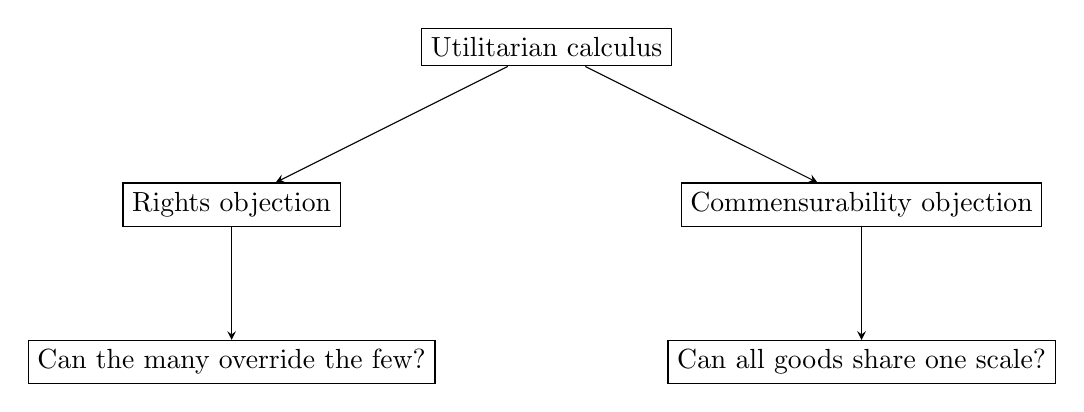
\begin{tikzpicture}[>=stealth]
\node[draw, rectangle] (u) at (0,2) {Utilitarian calculus};
\node[draw, rectangle] (r) at (-4,0) {Rights objection};
\node[draw, rectangle] (c) at (4,0) {Commensurability objection};
\node[draw, rectangle] (rr) at (-4,-2) {Can the many override the few?};
\node[draw, rectangle] (cc) at (4,-2) {Can all goods share one scale?};
\draw[->] (u) -- (r);
\draw[->] (u) -- (c);
\draw[->] (r) -- (rr);
\draw[->] (c) -- (cc);
\end{tikzpicture}
\end{figure}

The figure is only a map of the argument, but it captures Sandel's consolidation step exactly. The lecture is no longer dealing with scattered reactions. It has identified two precise pressure points in Bentham's theory.

\section{Bentham on Quantity, Not Quality}

At this point Sandel pushes one level deeper. Even if we set aside rights and even if we grant, for a moment, that values can be put on one scale, should every preference be counted without regard to its character? Bentham's answer is famously austere. What matters is quantity, not quality: intensity and duration, not nobility or baseness.

His slogan is that, the quantity of pleasure being equal, pushpin is as good as poetry. In a schematic notation we may write
\begin{equation}
\operatorname{Qty}(p_1)=\operatorname{Qty}(p_2)\Longrightarrow p_1\sim p_2.
\end{equation}
This is not a line Sandel writes on the board. It is the conceptual content of Bentham's claim. If two activities generate the same amount of pleasure, then they are equally good from the standpoint of utility.

There is something attractive here. The refusal to rank Mozart over Madonna, ballet over bowling, or one class's amusements over another class's pleasures can sound egalitarian and anti-paternalist. Bentham seems to spare us the arrogance of declaring other people's enjoyments intrinsically inferior.

And yet Sandel asks whether this nonjudgmental stance can really be sustained. The Roman crowd's pleasure in blood sport is not merely another entry in the pleasure column. It seems corrupt, base, degrading. The objection here is different from the rights objection. We may object not only because a victim is wronged, but because the crowd's pleasure is the wrong kind of pleasure to be counted in the first place. Once that thought appears, Bentham's flat metric begins to look unstable.

\section{Mill's Repair: Higher Pleasures and the Competent Judge}

John Stuart Mill now enters not as an enemy of utilitarianism but as its reformer. Sandel spends a few moments on the biographical setup because it helps explain Mill's ambition. Bentham's austere arithmetic passes through James Mill to John Stuart Mill, whose education was extreme, whose breakdown was severe, and whose mature philosophical project was to humanize utilitarianism without abandoning it.

Mill's first insistence is that utility remains the only standard of morality. He does not reject Bentham's premise. He accepts it. The question is whether that premise can be refined from within.

\begin{definition}
Mill's competent-judge test says that of two pleasures, the higher pleasure is the one that all or almost all who have experienced both decidedly prefer, and prefer independently of any external feeling of moral obligation.
\end{definition}

In a compact notation we may summarize the idea as
\begin{equation}
\text{Higher}(p_1,p_2)
\iff
\text{those acquainted with both }p_1\text{ and }p_2\text{ decidedly prefer }p_1.
\end{equation}
The force of the criterion lies in its restraint. Mill does not invoke an external standard. He stays within the field of desire. But he restricts the relevant desires to those of persons who know both sides of the comparison.

\subsection{Question \& Answer}

The question raised at this point is exactly the one Sandel places before the room:

\paragraph{}
How can a utilitarian distinguish higher from lower pleasures without stepping outside utilitarian premises?

\paragraph{}
Mill's answer is that we need not step outside preference; we need only refine whose preference counts. We should not compare poetry and pushpin by asking people unfamiliar with poetry. Nor should we compare the pleasures of cultivated reflection and immediate amusement by consulting only those who know one side. The judge must have experienced both.

\paragraph{}
This is a clever repair. It allows Mill to preserve utility while denying Bentham's flatness. But the repair is also fragile. If the class of judges must be educated, cultivated, and acquainted with higher things, then the distinction between reporting preferences and educating preferences becomes very thin. The lecture does not hide this difficulty. It exploits it.

\section{The Classroom Experiment, Rights, and the Limits of the Repair}

Sandel then turns the room into evidence. He shows three clips: a Hamlet soliloquy, an episode of \emph{Fear Factor}, and a clip from \emph{The Simpsons}. The first poll asks what the students like most. The second asks what they judge to be the highest or worthiest experience. The two questions are not the same, and the gap between them is the point:
\begin{equation}
\text{Preferred} \neq \text{Higher}.
\end{equation}

The result is striking. The class overwhelmingly prefers \emph{The Simpsons} to Shakespeare in immediate entertainment value. But when asked which experience is higher, the poll shifts toward Shakespeare. This is precisely the pattern Mill needs. The immediate favorite need not be the higher pleasure.

The discussion that follows sharpens the interpretation. One student suggests that Shakespeare may only seem higher because culture tells us that it is higher. Another replies that if one had to live with a single body of material for the rest of one's life, the richer and deeper work would sustain a fuller mental life. The rat example drives the contrast even further. Intense pleasure can be vivid and compelling; that does not make it the life one would choose over a lifetime.

Mill's most famous formula gathers the point: it is better to be a human being dissatisfied than a pig satisfied, better to be Socrates dissatisfied than a fool satisfied. Sandel does not present this as mere rhetoric. He presents it as Mill's attempt to show that some pleasures engage higher human faculties and are therefore preferred by those who know both.

Mill then tries the same strategy on rights and justice. Justice, he says, is not some mysterious non-utilitarian realm. It is the most sacred and binding part of morality because it stands higher in the scale of social utility. In a compact ordinal notation one might write
\begin{equation}
\text{Justice and rights} \succ \text{other moral requirements}.
\end{equation}
The meaning of the symbol is only comparative. Mill is not giving us a measured unit of justice. He is saying that, in the long run, a society that respects rights is better for progressive human beings than one that treats rights as easily tradable.

This is the lecture's last and deepest uncertainty. Has Mill truly repaired utilitarianism from within? Or has he quietly introduced standards that Bentham's original calculus could never generate on its own? Sandel does not answer decisively. He leaves the issue open, and the open question is the right ending.

The coda returns us to Bentham himself. Bentham's preserved body, his wax head, his literal posthumous usefulness: these details are not comic decoration alone. They show Sandel's final theme in miniature. Bentham is a philosopher who carried his own principle into life and death. The lecture ends not by dismissing him, but by showing how powerful and how strange that consistency can be.

\section{Summary}

We began with a simple rule:
\[
\text{maximize utility}.
\]
From that rule we derived a policy arithmetic:
\[
\text{add benefits, subtract costs, choose the larger balance}.
\]
The Czech smoking study and the Ford Pinto memo showed how this arithmetic actually functions when life and death enter the ledger. The objections then came into focus: perhaps utility fails to respect rights, and perhaps it presupposes a false commensurability among goods. Bentham answered by flattening quality into quantity. Mill answered by distinguishing higher from lower pleasures and by giving justice a privileged place within social utility. Whether Mill remains a utilitarian in the strict sense is the question Sandel leaves for the next stage of the course.